\documentclass[a4paper,11pt]{article}
\usepackage[polish]{babel}
\usepackage[OT4]{fontenc}
\usepackage[utf8]{inputenc}
\usepackage{graphicx}
\usepackage{subfig}
\usepackage{epstopdf}




\date{13/04/2014}


%opening
\title{PAMSI -- testowanie algorytmów wyszukiwania}
\author{Piotr Wilkosz}
\captionsetup{belowskip=12pt,aboveskip=4pt}
\begin{document}

\maketitle

\section{Wstęp}
Celem ćwiczenia było przetestowanie implementacji takich struktur danych jak:
  \begin{itemize}
   \item Tablica asocjacyjna - tworzenie z góry posortowanej tablicy i wyszukiwanie elementu
   \item Binarne drzewo przeszukiwań
   \item Tablica haszująca z adresowaniem liniowym
  \end{itemize}
Zadaniem było zmierzenie czasu wykonywania operacji wyszukania losowego elementu wśród powyższych struktur.
\section{Wyniki pomiarów}
\begin{enumerate}
 \item Tablica asocjacyjna
   
  \begin{table}[th]
  \centering
    \caption{Pomiar czasu wyszukania losowego elementu w tablicy asocjacyjnej}

      \begin{tabular}{|l|l|l|}
	\hline
	N & czas & odchylenie \\
    \hline
  10 & 6.7048e-06 &  3.49235e-06\\
  \hline
100 & 1.20477e-05 &  2.6002e-06\\
\hline
1000 & 1.74256e-05 &  2.58526e-06\\
\hline
10000 & 2.34596e-05 &  3.69745e-06\\
\hline
100000 & 3.92021e-05 &  4.56431e-06\\
\hline
200000 & 4.11365e-05 &  6.67398e-06\\
\hline
    \end{tabular}
    \end{table}
    \newpage
 \begin{figure}[th]
\centering
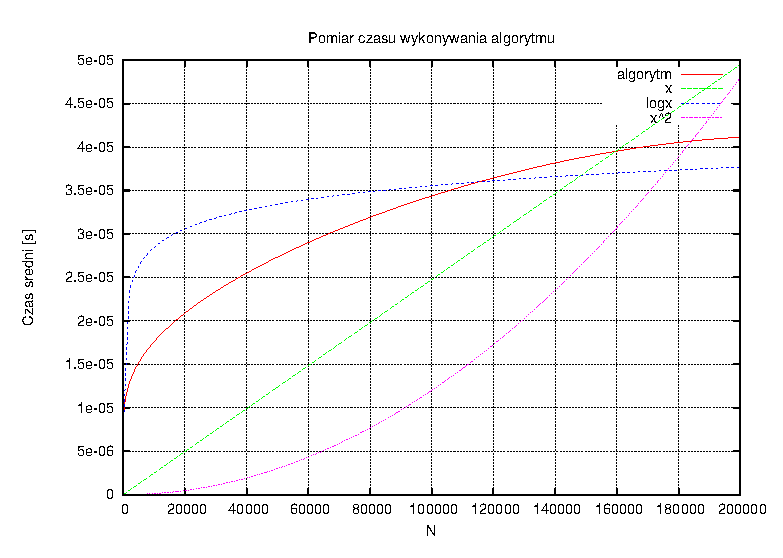
\includegraphics[width=0.8\textwidth]{../prj/wykres12.eps}
\caption{Wykres do tabeli nr 1}
\label{Wykres do tabeli nr 1}
\end{figure} 
Na podstawie wykresu złożoność obliczeniową operacji wyszukiwania w tablicy asocjacyjnej szacuje się na $ O(logn) $
\item Binarne drzewo przeszukiwań

  \begin{table}[th]
  \centering
  
    \caption{Pomiar czasu wyszukania losowego elementu w binarnym drzewie przeszukiwań}

      \begin{tabular}{|l|l|l|}
	\hline
	N & czas & odchylenie \\
    \hline
  10 & 8.5488e-06 &  3.08769e-06\\
  \hline
100 & 1.63919e-05 &  3.06447e-06\\
\hline
1000 & 2.26005e-05 &  3.77314e-06\\
\hline
10000 & 3.23784e-05 &  6.64965e-06\\
\hline
100000 & 4.77856e-05 &  8.44921e-06\\
\hline
1000000 & 6.9513e-05 &  8.87252e-06\\
\hline
    \end{tabular}
    \end{table}
    \newpage
\begin{figure}[th]
\centering
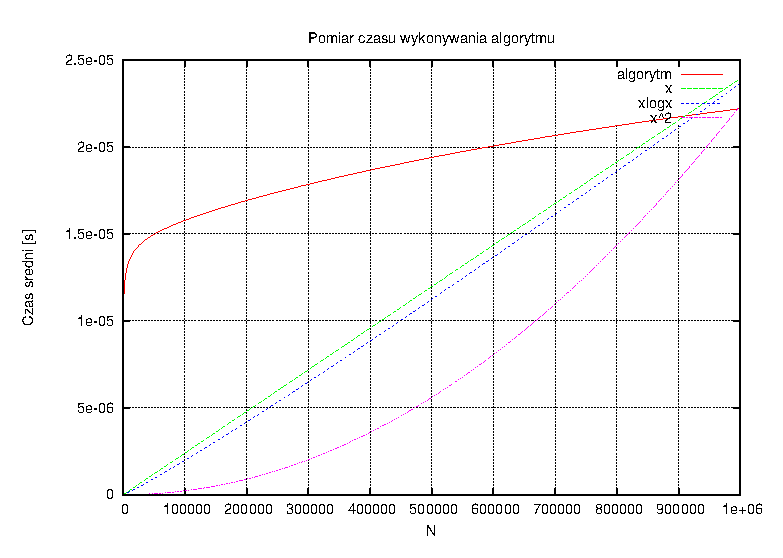
\includegraphics[width=0.8\textwidth]{../prj/wykres10.eps}
\caption{Wykres do tabeli nr 2}
\label{Wykres do tabeli nr 2}
\end{figure} 
Na podstawie wykresu złożoność obliczeniową operacji wyszukiwania w BST szacuje się na $ O(logn) $
\item Tablica haszująca

\begin{table}[th]
\centering
    \caption{Pomiar czasu wyszukania losowego elementu w tablic haszującej}

      \begin{tabular}{|l|l|l|}
	\hline
	N & czas & odchylenie \\
    \hline
  10 & 2.33365e-05 &  3.41544e-06\\
  \hline
100 & 5.06862e-05 &  7.05086e-06\\
\hline
1000 & 4.44422e-05 &  5.12816e-06\\
\hline
10000 & 5.34565e-05 &  8.91332e-06\\
\hline
100000 & 6.63957e-05 &  1.82487e-05\\
\hline
1000000 & 6.83327e-05 &  1.39888e-05\\
\hline
    \end{tabular}
    \end{table}
    \newpage
\begin{figure}[th]
\centering
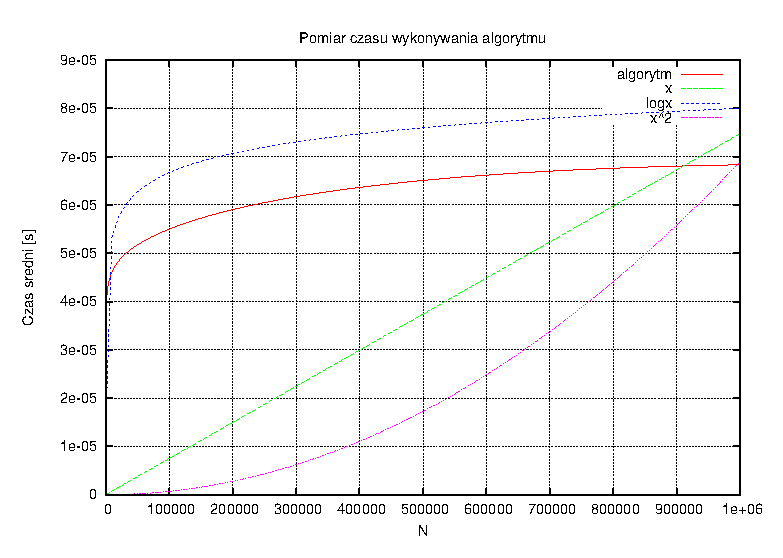
\includegraphics[width=0.8\textwidth]{../prj/wykres11.eps}
\caption{Wykres do tabeli nr 3}
\label{Wykres do tabeli nr 3}
\end{figure} 
Jak widać na wykresie, dla rosnącego rozmiaru problemu, złożoność dąży do $ O(1) $
\end{enumerate}

\section{Wnioski}

\begin{itemize}
\item Wszystkie przetestowane algorytmy cechują się dużą szybkością. Dla danych rzędu miliona czas wyszukiwania w każdej z powyższych struktur jest zadowalający, tzn. praktycznie 
niezauważalny dla pojedynczego wyszukania

\item Tablica asocjacyjna, bazująca na dwóch tablicach, została zaimplementowana w sposób umożliwiający przeszukiwanie binarne, czyli podczas wstawiania danych do
struktury są one jednocześnie sortowane. Jednakże tworzenie owej struktury jest czasochłonne, co jest sporą przeszkodą podczas prowadzenia testów
algorytmu, aczkolwiek jest dość wydajną strukturą, gdy dane nie są nazbyt często uzupełniane (problem długiego czasu tworzenia struktury wynika z
operacji porównania dwóch obiektów typu string, co znacząco ów czas wydłuża oraz z konieczności odpowiedniego gospodarowania pamięci). Złożoność obliczeniowa wyszukiwania: $ O(log_{2}n) $
\item Binarne drzewo przeszukiwań posiada podobne cechy, jak w przypadku poprzedniej struktury. Niewątpliwą zaletą jest prostsza implementacja, jednak w przeciwieństwie do powyższego algorytmu
istnieje ryzyko, iż złożoność obliczeniowa wyszukiwnia wyniesie $ O(n) $ (przypadek pesymistyczny). Oczekiwana złożoność wyszukiwania: $ O(log_{2}n) $
\item Tablica haszująca posiada oczekiwaną złożoność obliczeniową $ O(1) $. Podczas testów dla danych rzędu miliona, czas wyszukiwania stabilizował się dążąc do osiągnięcia wartości stałej, 
co jest oczywiste biorąc pod uwagę fakt, iż prawdopodobieństwo kolizji zmniejsza się wraz ze wzrostem rozmiaru tablicy. Pesymistyczny przypadek złożoności obliczeniowej wyszukiwania wynosi
$ O(n) $ jednak przy zastosowaniu odpowiedniej funkcji haszującej oraz dla dużych danych, algorytm taki jest o wiele szybszy od dwóch powyższych, co jest tym bardziej
widoczne, im większy jest rozmiar problemu. Czas tworzenia tablicy haszującej jest również o wiele krótszy w porównaniu z powyższymi algorytmami.
\end{itemize}
\end{document}
